%%%%%%%%%%%%%%%%%%%%%%%%%%%%%%%%%%%%%%%%%%%%%%%%%%%%%%%%%%%%
%%% LIVECOMS ARTICLE TEMPLATE FOR TRAINING ARTICLE
%%% ADAPTED FROM ELIFE ARTICLE TEMPLATE (8/10/2017)
%%%%%%%%%%%%%%%%%%%%%%%%%%%%%%%%%%%%%%%%%%%%%%%%%%%%%%%%%%%%
%%% PREAMBLE
\documentclass[9pt,training]{livecoms}
% Use the 'onehalfspacing' option for 1.5 line spacing
% Use the 'doublespacing' option for 2.0 line spacing
% Use the 'lineno' option for adding line numbers.
% Use the "ASAPversion' option following article acceptance to add the DOI and relevant dates to the document footer.
% Use the 'pubversion' option for adding the citation and publication information to the document footer, when the LiveCoMS issue is finalized.
% The 'training' option for indicates that this is a training article.
% Omit the bestpractices option to remove the marking as a LiveCoMS paper.
% Please note that these options may affect formatting.

\usepackage{lipsum} % Required to insert dummy text
\usepackage[version=4]{mhchem}
\usepackage{siunitx}
\DeclareSIUnit\Molar{M}
\usepackage[italic]{mathastext}
\graphicspath{{figures/}}

\usepackage{caption}
\usepackage{subcaption}

\newcommand{\kinA}{K}
\newcommand{\kinB}{K'}

\newcommand{\SeqA}{S}
\newcommand{\SeqB}{S'}

%%%%%%%%%%%%%%%%%%%%%%%%%%%%%%%%%%%%%%%%%%%%%%%%%%%%%%%%%%%%
%%% IMPORTANT USER CONFIGURATION
%%%%%%%%%%%%%%%%%%%%%%%%%%%%%%%%%%%%%%%%%%%%%%%%%%%%%%%%%%%%

\newcommand{\versionnumber}{1.0}  % you should update the minor version number in preprints and major version number of submissions.
\newcommand{\githubrepository}{\url{https://github.com/volkamerlab/kinase_similarity_pipeline_paper}}  %this should be the main github repository for this article

%%%%%%%%%%%%%%%%%%%%%%%%%%%%%%%%%%%%%%%%%%%%%%%%%%%%%%%%%%%%
%%% ARTICLE SETUP
%%%%%%%%%%%%%%%%%%%%%%%%%%%%%%%%%%%%%%%%%%%%%%%%%%%%%%%%%%%%
\title{Kinase similarity assessment pipeline for off-target prediction [Article v\versionnumber]}

\author[1\authfn{1}]{Talia B. Kimber}
\author[1\authfn{1}\authfn{2}]{Dominique Sydow}
\author[1*]{Andrea Volkamer}
\affil[1]{\textit{In silico} Toxicology and Structural Bioinformatics, Institute of Physiology, Charit\'e-Universit\"atsmedizin Berlin, Charit\'eplatz 1, 10117, Berlin, Germany}

\corr{andrea.volkamer@charite.de}{AV}

\orcid{Talia B. Kimber}{0000-0002-8881-920X}
\orcid{Dominique Sydow}{0000-0003-4205-8705}
\orcid{Andrea Volkamer}{0000-0002-3760-580X}

\contrib[\authfn{1}]{These authors contributed equally to this work}

\presentadd[\authfn{2}]{Sosei Heptares, Steinmetz Building, Granta Park, Cambridge CB21 6DG, United Kingdom}

\blurb{This LiveCoMS document is maintained online on GitHub at \githubrepository; to provide feedback, suggestions, or help improve it, please visit the GitHub repository and participate via the issue tracker.}

%%%%%%%%%%%%%%%%%%%%%%%%%%%%%%%%%%%%%%%%%%%%%%%%%%%%%%%%%%%%
%%% PUBLICATION INFORMATION
%%% Fill out these parameters when available
%%% These are used when the "pubversion" option is invoked
%%%%%%%%%%%%%%%%%%%%%%%%%%%%%%%%%%%%%%%%%%%%%%%%%%%%%%%%%%%%
\pubDOI{10.XXXX/YYYYYYY}
\pubvolume{<volume>}
\pubissue{<issue>}
\pubyear{<year>}
\articlenum{<number>}
\datereceived{Day Month Year}
\dateaccepted{Day Month Year}

%%%%%%%%%%%%%%%%%%%%%%%%%%%%%%%%%%%%%%%%%%%%%%%%%%%%%%%%%%%%
%%% ARTICLE START
%%%%%%%%%%%%%%%%%%%%%%%%%%%%%%%%%%%%%%%%%%%%%%%%%%%%%%%%%%%%

\begin{document}

\begin{frontmatter}
\maketitle

\begin{abstract}
Kinases are established drug targets to combat cancer and inflammatory diseases. Despite decades of kinase research, challenges still remain, such as the under-exploration of a large fraction of the kinome and the promiscuous binding of many kinase inhibitors. Due to the highly conserved ATP binding site in kinases, ligands may bind not only to their designated kinase (on-target) but also to other kinases (off-targets). Such promiscuous binding can cause mild to severe side effects, and the prediction of these off-targets is highly non-trivial.
Therefore, we propose a pipeline that allows the study of kinase similarities from four different angles in an automated and modular fashion. The first method considers the binding site sequence. The second method uses structural information via KiSSim, a newly developed fingerprint that considers both physico-chemical and spatial properties of the binding site. The third method involves kinase-ligand interaction fingerprints as provided by KLIFS, and the last method utilizes the measured activity of ligands on kinases based on ChEMBL data. Finally, results for a given set of kinases are collected and analyzed to gain insight into potential off-targets from the different aforementioned perspectives. Since the pipeline is set up as a series of Jupyter notebooks covering both theoretical and practical aspects, the target audience ranges from beginners to advanced users working in the field of natural and computer sciences. The pipeline is part of the TeachOpenCADD project and extends it with this special kinase edition.
\end{abstract}

\end{frontmatter}

\section{Introduction}
Kinases are involved in most cellular processes by phosphorylating\textemdash and thereby activating\textemdash themselves or other proteins. This family is among the most frequently mutated proteins in tumors and has been successfully studied as drug targets for many decades~\cite{Cohen_2021_NatRevDrugDiscov}. Thanks to the longstanding research, a plethora of kinase data is freely available, i.e. as part of databases such as UniProt~\cite{uniprot_consortium_2020_nar}, PDB~\cite{Berman_2000_NAR} or ChEMBL~\cite{Gaulton_2016_nar}, and has been made easily accessible via kinase resources such as the KLIFS\textemdash Kinase-Ligand Interaction Fingerprints and Structures\textemdash database~\cite{Kanev_2020_NAR}. As of February 2022, $5\,911$ X-ray structures of human kinases have been resolved (see the KLIFS database~\cite{klifs_feb_2022}) and $70$ FDA-approved small molecule protein kinase inhibitors are on the market~\cite{FDA_PKI_2022}. Most of the approved drugs bind in the ATP-binding pocket and intermediate surroundings.

Although structural information provides rich information, kinases have been widely classified based on sequence. \citet{Manning_2022_science} clustered the human protein kinases based on their sequence similarity into eight major groups (AGC, CAMK, CK1, CMGC, RGC, STE, TK, TKL) and one “Other” group for unassigned kinases, as well as atypical kinases. The resulting Manning kinome tree depicts kinase clustering (see Figure~\ref{fig:kinmap}).

Despite decades of kinase research, challenges still remain~\cite{Kooistra_2017_AnnualReportsMedicinalChemistry}. For example: \begin{enumerate}
    \item A large fraction of the kinome is un-/underexplored. Figure~\ref{fig:structure_per_kinase} shows the number of PDB structures per kinase, unveiling a vast imbalance between structurally resolved kinases and unexplored ones. For example, CDK2 has been resolved in $426$ PDB structures, while only $313$ kinases~\cite{klifs_feb_2022} out of approximately $540$ in the kinome~\cite{Kooistra_2017_AnnualReportsMedicinalChemistry} have been structurally resolved.
    \item Many kinase inhibitors are promiscuous binders causing off-target effects or enabling polypharmacology. For example, the Epidermal Growth Factor Receptor~(EGFR) inhibitor Erlotinib shows affinities to other kinases in the highly sequentially-similar TK kinase group, but also strongly affects off-targets in more remote kinase groups (see Figure\ref{fig:off_target}).
\end{enumerate}

Therefore, assessing kinase similarity from different angles may be a crucial step in understanding and predicting off-targets to help designing more selective drugs and avoiding side effects.

\subsection{Scope}
In this study, similarities between a set of kinases are investigated based on methods offering different perspectives on this challenging topic, as summarized in Table~\ref{tab:notebook_overview}. The first method considers the binding site sequence as deposited in the KLIFS database. The second method uses KiSSim~\cite{sydow_2021_kissim_chemrxiv}, a recently developed fingerprint that considers physico-chemical as well as spatial properties of the binding site. The third method involves protein-ligand interaction fingerprints as provided in the KLIFS database, and the last method utilizes the measured activity of ligands against kinases based on ChEMBL data~\cite{Gaulton_2016_nar}. The different methods are preceded by a general introduction to kinases and the challenges faced during kinase-centric drug design, and succeeded by a comparison between the different kinase similarity methods.

Moreover, this study has been put together into a modular pipeline that enables the research of kinase similarities in an automated fashion, allowing users to simply use it out of the box, or adapt it to their needs.

\begin{table*}
    \centering
    \begin{tabular}{p{0.25\textwidth}p{0.55\textwidth}p{0.1\textwidth}}
    \hline
    \textbf{Topic} & \textbf{Description} & \textbf{Hyperlink} \\
    \hline
    \hline
    What is a kinase? & Introduction to kinases and challenges in drug discovery. & \href{https://projects.volkamerlab.org/teachopencadd/talktorials/T023\_what\_is\_a\_kinase.html}{T023} \\
    Pocket sequence & Pairwise similarities/identities between $85$ residue long KLIFS pocket sequences. & \href{https://projects.volkamerlab.org/teachopencadd/talktorials/T024\_kinase\_similarity\_sequence.html}{T024} \\
    Pocket structure & Pairwise similarities between $1032-$bit long KiSSim fingerprints, which encode spatial and physico-chemical pocket properties. & \href{https://projects.volkamerlab.org/teachopencadd/talktorials/T025\_kinase\_similarity\_kissim.html}{T025} \\
    Pocket-ligand interactions & Pairwise similarities between $595-$bit long KLIFS kinase-ligand interaction fingerprints (IFP). & \href{https://projects.volkamerlab.org/teachopencadd/talktorials/T026\_kinase\_similarity\_ifp.html}{T026} \\
    Ligand profile & Similarity based on the ratio of compounds tested active against kinase pairs.& \href{https://projects.volkamerlab.org/teachopencadd/talktorials/T027\_kinase\_similarity\_ligand\_profile.html}{T027} \\
    Kinase similarity comparison & Comparison of predicted off-targets based on calculated kinase similarities using aforementioned methods. & \href{https://projects.volkamerlab.org/teachopencadd/talktorials/T028\_kinase\_similarity\_compare\_perspectives.html}{T028} \\
    \hline
\end{tabular}
    \caption{TeachOpenCADD kinase edition overview: Notebook topics, description, and index with a hyperlink to the associated notebook.}
    \label{tab:notebook_overview}
\end{table*}

\begin{figure}
     \centering
     \begin{subfigure}[b]{0.2\textwidth}
         \centering
         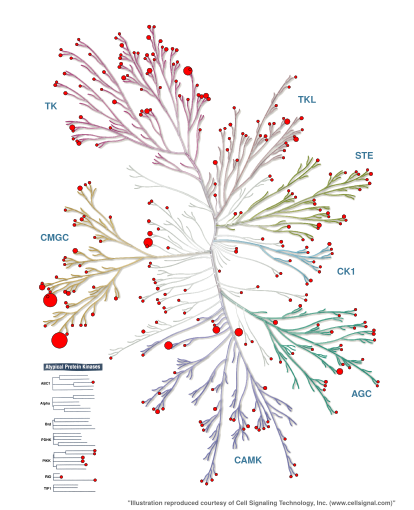
\includegraphics[width=\textwidth]{kinmap_n_structures_per_kinase.png}
         \caption{Number of PDB structures per kinase. The figure shows the imbalance between highly explored kinases, e.g. groups: TK, CMGC, and CAMK, and less explored ones, e.g. the CK1 group. CDK2 has the most structures ($426$). The red circle is proportional to the number of PDB structures, such that the greater is the circle, the higher is the number of structures.}
         \label{fig:structure_per_kinase}
     \end{subfigure}
     \hfill
     \begin{subfigure}[b]{0.2\textwidth}
         \centering
         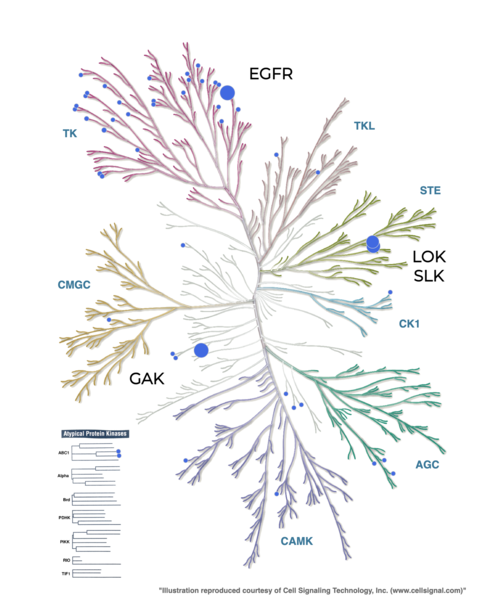
\includegraphics[width=\textwidth]{kinmap_erlotinib_karaman.png}
         \caption{Developing selective kinase inhibitors is non-trivial since kinases are highly conserved in the ATP binding site. EGFR inhibitor Erlobinib binds not only to its intended target EGFR, but also to kinases in remote groups, such as SLK/LOK in the STE group and GAK in the CMGC group. The blue circle is proportional to the $K_d$ value in \SI{}{\nano\Molar} taken from the \citet{Karaman_2008_NatBiotechnol} dataset.}
         \label{fig:off_target}
     \end{subfigure}
        \caption{Visual representation using the Manning tree of existing challenges in kinase research: un-/underexplored kinase groups (left) and the promiscuity character of kinases (right). The figure is taken from \href{https://projects.volkamerlab.org/teachopencadd/}{https://projects.volkamerlab.org/teachopencadd/} and is generated using KinMap~\cite{Eid_2017_BMCBioinformatics}.}
        \label{fig:kinmap}
\end{figure}

\section{Prerequisites}
\subsection{Target audience}
The notebooks were developed to support researchers interested in kinase-centric computational drug design with a focus on understanding and predicting kinase off-targets. 
As this collection is part of the TeachOpenCADD~\cite{Sydow_2019_JCheminform, Sydow_2021_toc_chemrxiv} training material, we also recommend the notebooks to teachers as pedagogical interactive material in structural bioinformatics and cheminformatics.

\subsection{Background knowledge}
The notebooks are constructed in a way that no in depth prior knowledge besides an affinity for the natural or computer sciences is required. Each notebook eases into the topic of kinase drug development and kinase similarity with a lot of theoretical background and comments on all content as well as programming-related steps in great detail. Nevertheless, users will benefit from a basic understanding of the Python programming language and the usage of Jupyter notebooks. If such basic introduction is needed, please refer to training material as listed on the TeachOpenCADD website~\cite{toc_python_2022}.

\subsection{Software requirements}
The notebooks are written in Python and rely on open-source packages such as pandas~\cite{pandas_2020}, numpy~\cite{harris_2020_numpy}, scipy~\cite{Virtanen_2020_NMeth}, matplotlib~\cite{Hunter_2007_IEEE}, seaborn~\cite{Waskom_2021_seaborn}, scikit-learn~\cite{Pedregosa_2011_JMLR}, rdkit~\cite{RDKit_2022}, biotite~\cite{Kunzmann_2018_biotite}, opencadd~\cite{Sydow_2022_JOSS}, requests~\cite{requests_2022}, and pillow~\cite{pillow_2022}.

The user only needs to install the \textit{teachopencadd} conda-forge package~\cite{toc_conda_forge_2022} (see installation~\cite{toc_website_installing}), which will install all relevant packages and save a copy of all TeachOpenCADD notebooks\textemdash including the kinase edition discussed in this paper\textemdash on the user's local machine. A read-only mode of the notebooks is accessible via the TeachOpenCADD website at \href{https://projects.volkamerlab.org/teachopencadd/}{https://projects.volkamerlab.org/teachopencadd/}.

\section{Method}
\label{sec:method}
In this section, the four methods that are introduced to quantify kinase similarity are described, namely the pocket sequence, the KiSSim fingerprint, the interaction fingerprint, and the ligand profile. Note that the theoretical and practical aspects of each method are also covered in great detail in the individual notebooks of this kinase collection (Table~\ref{tab:notebook_overview}).

\subsection{Pocket sequence}
The full amino acid sequence is often used to assess similarities between kinases (see the phylogenetic tree developed by \citet{Manning_2022_science}). Since binding sites are often more conserved than the whole protein, \citet{van_Linden_2013_JMedChem} defined as part of KLIFS a $85$-long pocket sequence that is aligned across the kinome. Using a sequence that focuses on the binding site seems appropriate in the case of kinases, since this is where the ligand is likely to bind. Moreover, working with a fixed length sequence is practical from a computational point of view. 

In this study, two methods are used to compute relationships based on sequence, namely the sequence identity and the sequence similarity, which are described below. 

\subsubsection{Sequence identity}
\begin{subequations}
The pairwise sequence identity, or simply sequence identity, is a similarity based on character-wise discrepancy, in other terms, the number of residues that match in two aligned sequences~\cite{Rost_1999_ProteinEngDesSel}.
More formally, given two kinase sequences \SeqA{} and \SeqB{} of same lengths $L$, the sequence identity can be defined as

\begin{equation}
    \text{sequence identity(\SeqA{}, \SeqB{})} = \frac{1}{L} \sum_{n=1}^{L} I\big(\SeqA[n], \SeqB[n]\big),
\end{equation}

where $I$ is the identity matrix of the amino acids, and $\SeqA[n]$ the amino acid at position $n$ of the kinase sequence $\SeqA$. Note that not all kinases have residues present at each of the 85 alignment positions. Such gaps are represented by "-" and count as mismatch to any amino acid.

\subsubsection{Sequence similarity}
Unlike sequence identity which treats all residues uniformly, pairwise sequence similarity, or sequence similarity, takes into account the change of the amino acids over evolutionary time, thus reflecting relationships between amino acids. It is based on a substitution matrix $M$, where each entry gives a score between two amino acids. In this study, the BLOSUM substitution matrix~\cite{Henikoff_1992_PNAS}, as implemented in biotite~\cite{Kunzmann_2018_BMC}, is used. Formally, the following is defined:

\begin{equation}
    \text{sequence similarity(\SeqA{}, \SeqB{})} = \frac{1}{L} \sum_{n=1}^{L} M'\big(\SeqA[n], \SeqB[n]\big), 
\end{equation}

where $M'$ is the translated and rescaled version of the substitution matrix $M$.
\end{subequations}

For both the sequence identity and similarity, the closer the value is to $1$, the more similar are the kinases.

Figure~\ref{fig:pocket_sequence} shows the sequence similarity between the KLIFS pocket sequence of EGFR and MET kinases. Sequence similarity is used by default in the pipeline for further analysis.

\begin{figure}[ht]
    \centering
    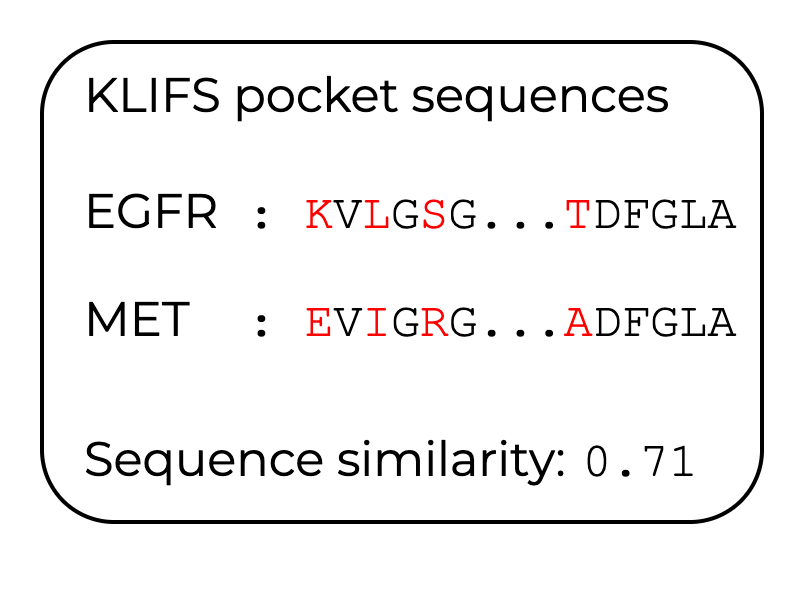
\includegraphics[width=0.5\columnwidth]{sequence_similarity.png}
    \caption{Sequence similarity between EGFR and MET. The $85$ residue pocket sequence is retrieved from KLIFS. The pairwise sequence similarity takes into account the change of the amino acids over evolutionary time.}
    \label{fig:pocket_sequence}
\end{figure}

\subsection{The KiSSim fingerprint}
In order to assess the pairwise similarity of kinases from a structural point of view, the newly developed KiSSim (\textbf{Ki}nase \textbf{S}tructure \textbf{Sim}ilarity) fingerprint~\cite{sydow_2021_kissim_chemrxiv, kissim_package} is used. This fingerprint describes the physico-chemical and spatial properties of structurally resolved kinases, while focusing on the KLIFS pocket residues. Each structure is mapped to a fingerprint composed of $1032$ bits, the first $680 \, (=85 \times 8)$ describing physico-chemical features and the remaining $352 \, (=85 \times 4 + 12)$ spatial information (see Figure~\ref{fig:kissim_similarity}).

\begin{figure}[ht]
    \centering
    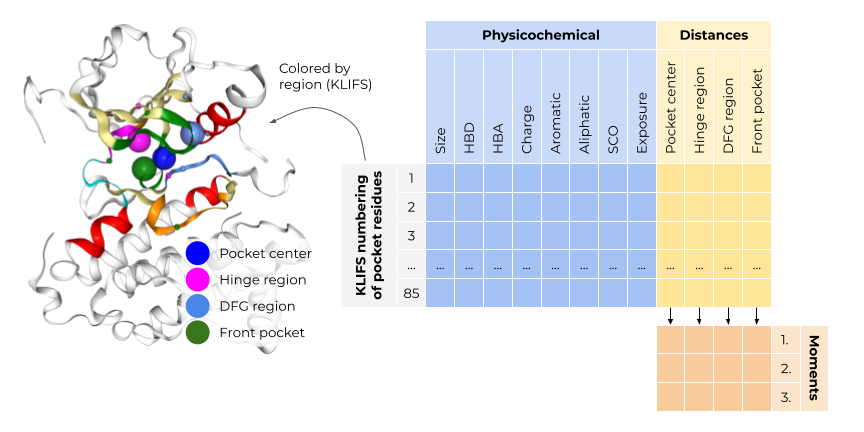
\includegraphics[width=\columnwidth]{kissim_fingerprint.png}
    \caption{The $1032$-long KiSSim fingerprint encodes physico-chemical and spatial properties of the kinase's pocket, adding a structural perspective on kinases. The figure is adapted from \cite{kissim_package}.}
    \label{fig:kissim_similarity}
\end{figure}

\subsubsection{From several structures to one kinase}

A kinase can be represented by one or even a hundred resolved crystal structures in the PDB (see Figure~\ref{fig:structure_per_kinase}). In this study, we aim at comparing different kinases and not individual structures. Since KiSSim generates a fingerprint for each structure, the following mapping from structures to kinase is applied:

Given two kinases \kinA{} and \kinB{}, all available structures in KLIFS for these kinases are fetched using opencadd~\cite{Sydow_2022_JOSS}, namely $s_1, \dots, s_m$ for kinase \kinA, and $s'_1, \dots, s'_n$ for kinase \kinB, noting that the number of structures might be different for each kinase. Each structure $s_i, s'_i$ is then mapped to its corresponding KiSSim fingerprint $fp_i, fp'_i$, see Figure~\ref{fig:structure_to_kinase}. The fingerprints fp, fp' corresponding to kinases \kinA{}, \kinB{} respectively, are the ones for which the Euclidean distance is minimized (Figure~\ref{fig:structure_to_kinase}). Note that these \textit{minimal distance} fingerprints vary for each kinase depending on the compared \kinA{}, \kinB{} pair.

\begin{figure}[ht]
    \centering
    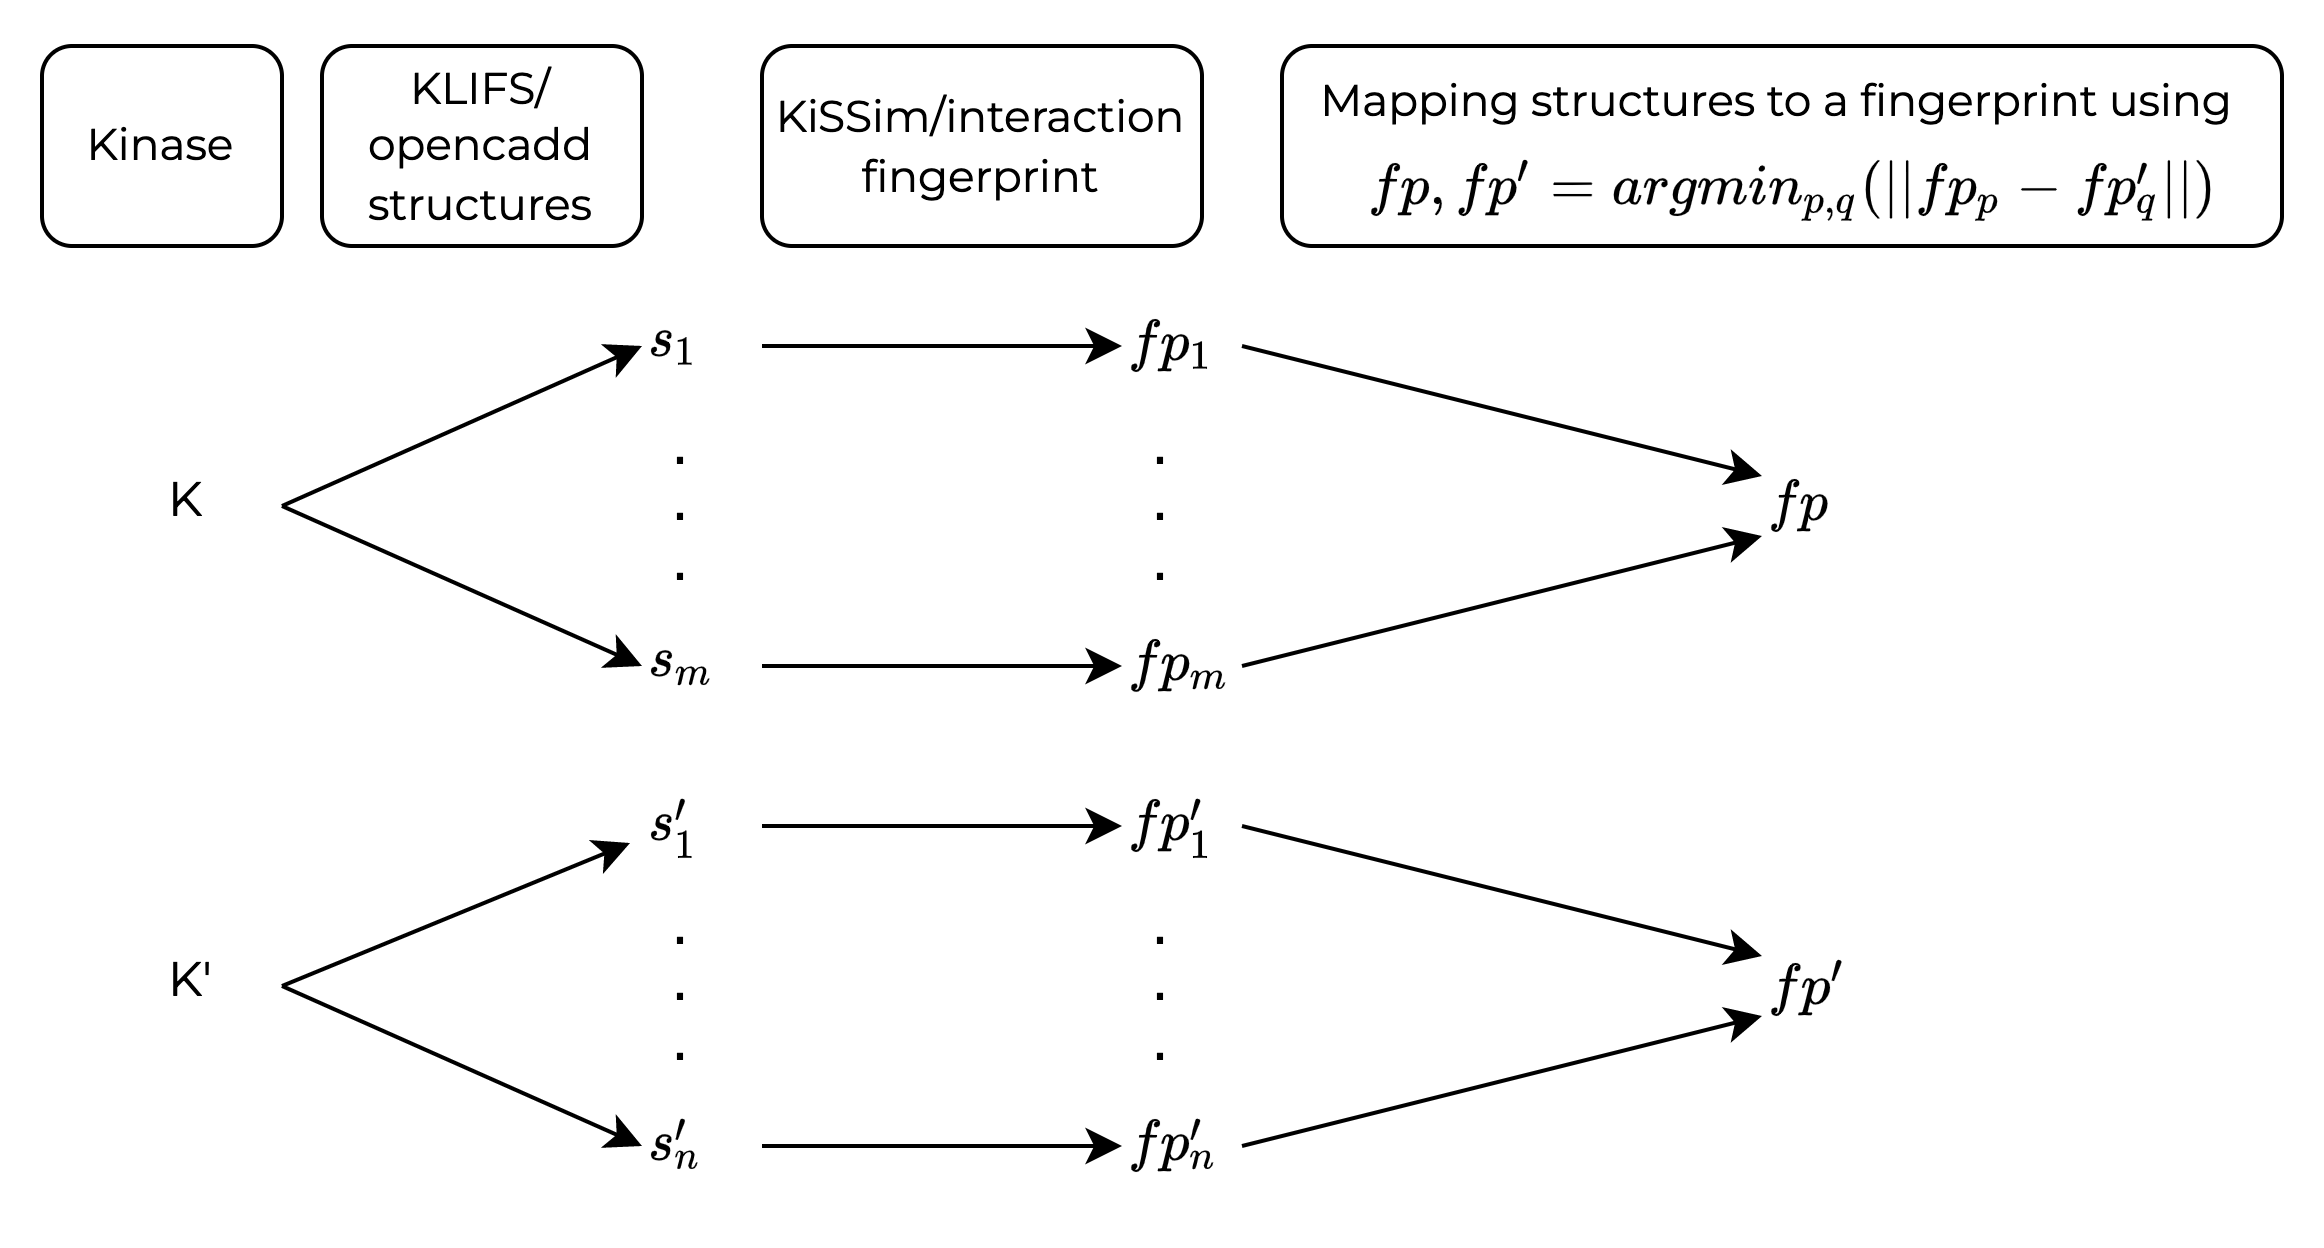
\includegraphics[width=\columnwidth]{structure_to_kinase.png}
    \caption{Associating one structural fingerprint per kinase. All available structures are retrieved for two given kinases and all fingerprints are computed. The fingerprints selected to be associated with the kinase in the present kinase pair are the ones for which the computed distance is minimized.}
    \label{fig:structure_to_kinase}
\end{figure}

Finally, two kinases \kinA{}, \kinB{} are compared based on their respective \textit{minimal distance} between KiSSim fingerprint fp, fp' using the Euclidean norm:

\begin{equation}
    \text{KiSSim dissimilarity (fp, fp')} = \left\lVert\text{fp} - \text{fp'}\right\rVert_2.
\end{equation}
In this case, the closer the value to $0$, the more similar the kinases.

\subsection{The interaction fingerprint}
Interaction fingerprints~(IFPs) encode the binding mode of a ligand in a binding site, i.e., the protein-ligand interactions that are present in a structurally resolved complex. If a ligand can form similar interaction patterns in proteins other than its designated protein (off- vs. on-target), it is possible that this ligand will cause unintended side effects. Knowledge about binding mode similarities can therefore help to avoid such off-target effects.
% ; or to exploit the known similarities for polypharmacology effects where one ligand could intentionally target multiple proteins at once.

The KLIFS interaction fingerprint describes seven possible interactions for each of the $85$ residues in the binding pocket. Interactions include
\begin{enumerate*}
    \item hydrophobic contacts,
    \item aromatic interactions, face to face,
    \item aromatic interactions, edge to face,
    \item H-bond donors,
    \item H-bond acceptors,
    \item cationic interactions, and
    \item anionic interactions. 
\end{enumerate*}
The $595$-bit long vector describes the presence or absence of such interactions for all $85$ residues (see Figure~\ref{fig:ifp_similarity}).

\begin{figure}[ht]
    \centering
    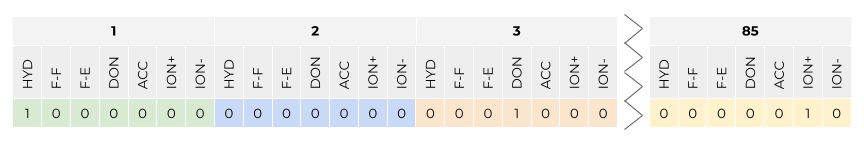
\includegraphics[width=\columnwidth]{IFP.png}
    \caption{The KLIFS interaction fingerprint encodes seven interaction types for each of the $85$ residues in the binding site. Interaction types include: hydrophobic contacts~(HYD), face to face aromatic interactions~(F-F), face to edge aromatic interactions~(F-E), protein H-bond donors~(DON), protein H-bond acceptors~(ACC), protein cationic interactions~(ION+), and protein anionic interactions~(ION-). The figure is taken from \cite{toc_website}.}
    \label{fig:ifp_similarity}
\end{figure}

Similarly to the KiSSim comparison, given two kinases \kinA{} and \kinB{}, all available structures in KLIFS for these kinases are fetched using opencadd~\cite{Sydow_2022_JOSS}. Each structure is mapped to its corresponding IFP. The interaction fingerprints fp, fp' corresponding to kinases \kinA{}, \kinB{} respectively are the ones for which the Jaccard distance~\cite{Kosub_2019_jpatrec} is minimized (Figure~\ref{fig:structure_to_kinase}). Note that the Euclidean distance is used in case of the KiSSim fingerprint, which contains continuous and discrete values, while the Jaccard distance is employed in case of the binary IFPs.

Finally, two kinases \kinA{}, \kinB{} are compared using their respective \textit{minimal distance} between interaction fingerprint fp, fp' and calculating the Jaccard distance:

\begin{equation}
    \text{IFP dissimilarity (fp, fp')} = d_J(\text{fp}, \text{fp'}),
\end{equation}
where $d_J$ is the Jaccard distance.

In this case, the closer the value to $0$, the more similar the kinases.

\subsection{Ligand profile}
In the context of drug design, the following assumption is often made: if a compound was tested active on two different kinases, it is suspected that these two kinases may have some degree of similarity~\cite{Barelier_2015_ACSChemBio}. This is the rationale behind the ligand profile similarity.
Given bioactivity data for a set of compounds measured against a set of targets\textemdash in this case kinases\textemdash and two kinases \kinA{}, \kinB{}, ligand profile similarity is defined as

\begin{equation}
    \text{lig. profile similarity(\kinA{}, \kinB{})} = \\
\frac{
    \#\text{ actives on both \kinA{} and \kinB{}}}
    {\#\text{ tested on both \kinA{} and \kinB{}}
    }.
\end{equation}

The closer the value is to $1$, the more similar are the kinases.
If no compounds were commonly tested on two kinases, then the similarity is set to $0$.
Computing the similarity between a kinase and itself may be interpreted as kinase promiscuity, where the similarity described above would therefore represent the fraction of active compounds over all tested compounds for this kinase.

\subsubsection{Bioactivity data}
The bioactivity data used for this method comes from Kinodata~\cite{kinodata_2022}, from the Openkinome organization~\cite{openkinome_feb_2022}. It is a pre-processed kinase subset of the ChEMBL data~\cite{Gaulton_2016_nar}, version 29. Further processing includes keeping only $IC_{50}$ values given in \SI{}{\nano\Molar}, and converted to $pIC_{50}$s. If there are several measurements for a kinase-compound pair, then the most active value, i.e. the entry with the highest $pIC_{50}$, value is kept. Finally, the $pIC_{50}$ values are binarized using a $6.3$ cutoff to discriminate between an active or inactive compound as described in~\cite{Merget_2017_JMedChem}. 

In the pipeline, one can additionally compute the non-reduced ratio of number of active compound against the total number of compounds to gain insight into the actual number of measurements for each kinase pair.

\subsection{Kinase comparison and clustering}
\label{sec:comparison}
To assess kinase similarities based on the calculated (dis)similarity matrices, two visualization methods are used, namely heatmaps and dendrograms.

\subsubsection{Heatmaps}
The heatmaps are generated using Matplotlib~\cite{Hunter_2007_IEEE} to depict the similarity between a set of kinases. The maximum value is $1$, indicating exact similarity, as is the case for diagonal entries. The value $0$ indicates total dissimilarity. Plotting such figures allows to see and extract patterns thanks to the gradient of colors, see top row in Figure~\ref{fig:comparison}.

\subsubsection{Dendrograms}
Clustering algorithms are used to identify groups such that the similarities within clusters are higher than compared to other clusters~\cite{Hastie_2009_ESLii}. In this study, hierarchical clustering is used, and, unlike heatmaps, it is based on distance (or dissimilarity).
% According to \citet{Hastie_2009_ESLii}, "The goal of cluster analysis is to partition the observations into groups (“clusters”) so that the pairwise dissimilarities between those assigned to the same cluster tend to be smaller than those in different clusters." 
Hierarchical clustering can be graphically displayed using a dendrogram (see bottom row in Figure~\ref{fig:comparison}), where the height of each node is proportional to the dissimilarity between its two daughter clusters.
% the height of each node is proportional to the value of the intergroup dissimilarity between its two daughters.
The clustering and plotting is done using Scikit-learn~\cite{Pedregosa_2011_JMLR} and Matplotlib~\cite{Hunter_2007_IEEE}, respectively.

\begin{figure*}
    \centering
    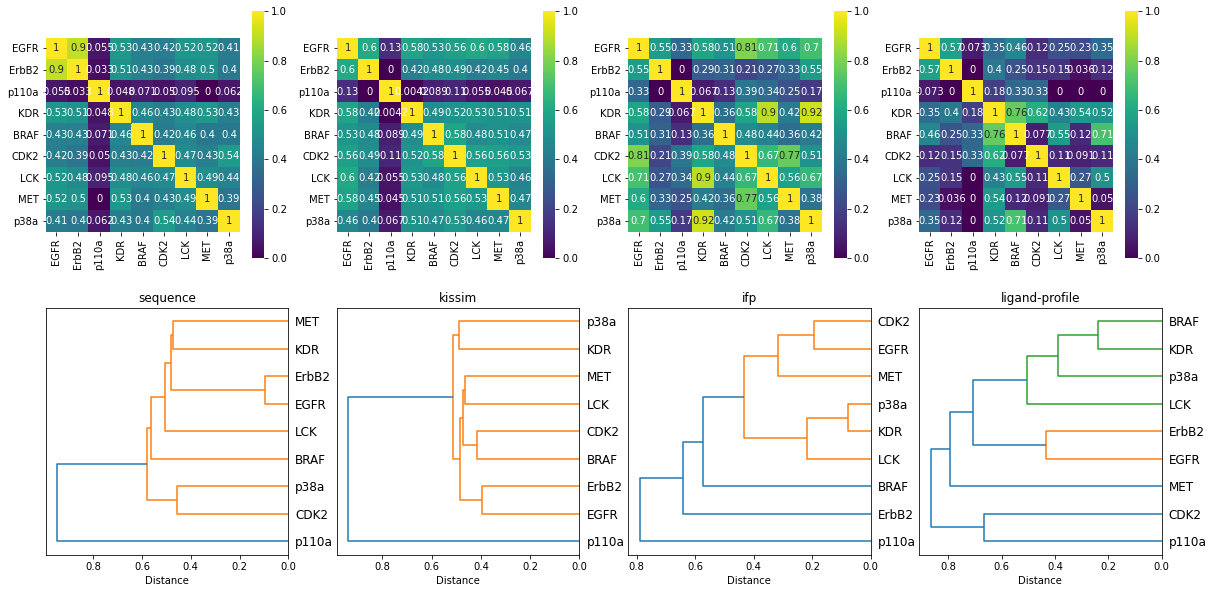
\includegraphics[width=\textwidth]{all_comparison.png}
    \caption{Visualization for kinase similarity from for different angles: sequence, KiSSim, interaction fingerprint~(ifp) as well as ligand profile. The top, bottom row shows four heatmaps, dendrograms respectively for a set of nine study kinases.}
    \label{fig:comparison}
\end{figure*}

For fair comparison, the distance matrices for all four methods are normalized so that each entry lives between $0$ and $1$. Similarity matrices\textemdash as used for the heatmaps\textemdash are then computed using $1-$distance matrix.

\section{Pipeline}
Measuring kinase similarity is a non-trivial task; distinct measures can provide different insights, which can be complementary, confirmatory, or contradictory, and therefore expand our knowledge on the target(s) at hand. 
However, implementing multiple methods can be time-consuming and comparing results across many output types can be laborious.
Turning such processes into a functional pipeline helps to avoid the scattering of scripts and to speed up iterations of the design-make-test-analyze cycle~\cite{Schneider_2019_NatRevDrugDiscov} of drug design campaigns. Moreover, following the findable, accessible,
interoperable, and reusable (FAIR) principles~\cite{Wilkinson_2016_SciData} makes such pipelines long-lasting and available to the community.

In the pipeline presented herein, we implement the different methods once and streamline each method's results into a standardized output with a pre-defined set of visualization tools for easy comparison, while leaving the pipeline flexible enough so that adding new methods or new visualization tools is effortless, making the whole process easy to understand, maintain, and expand.

\subsection{Means of the pipeline}
The proposed pipeline is a collection of six Jupyter notebooks~\cite{Kluyver_2016_Jupyter} that allows the study of kinase similarities from four different angles in an automated and modular fashion (Figure~\ref{fig:pipeline}).

\begin{figure}[ht]
    \centering
    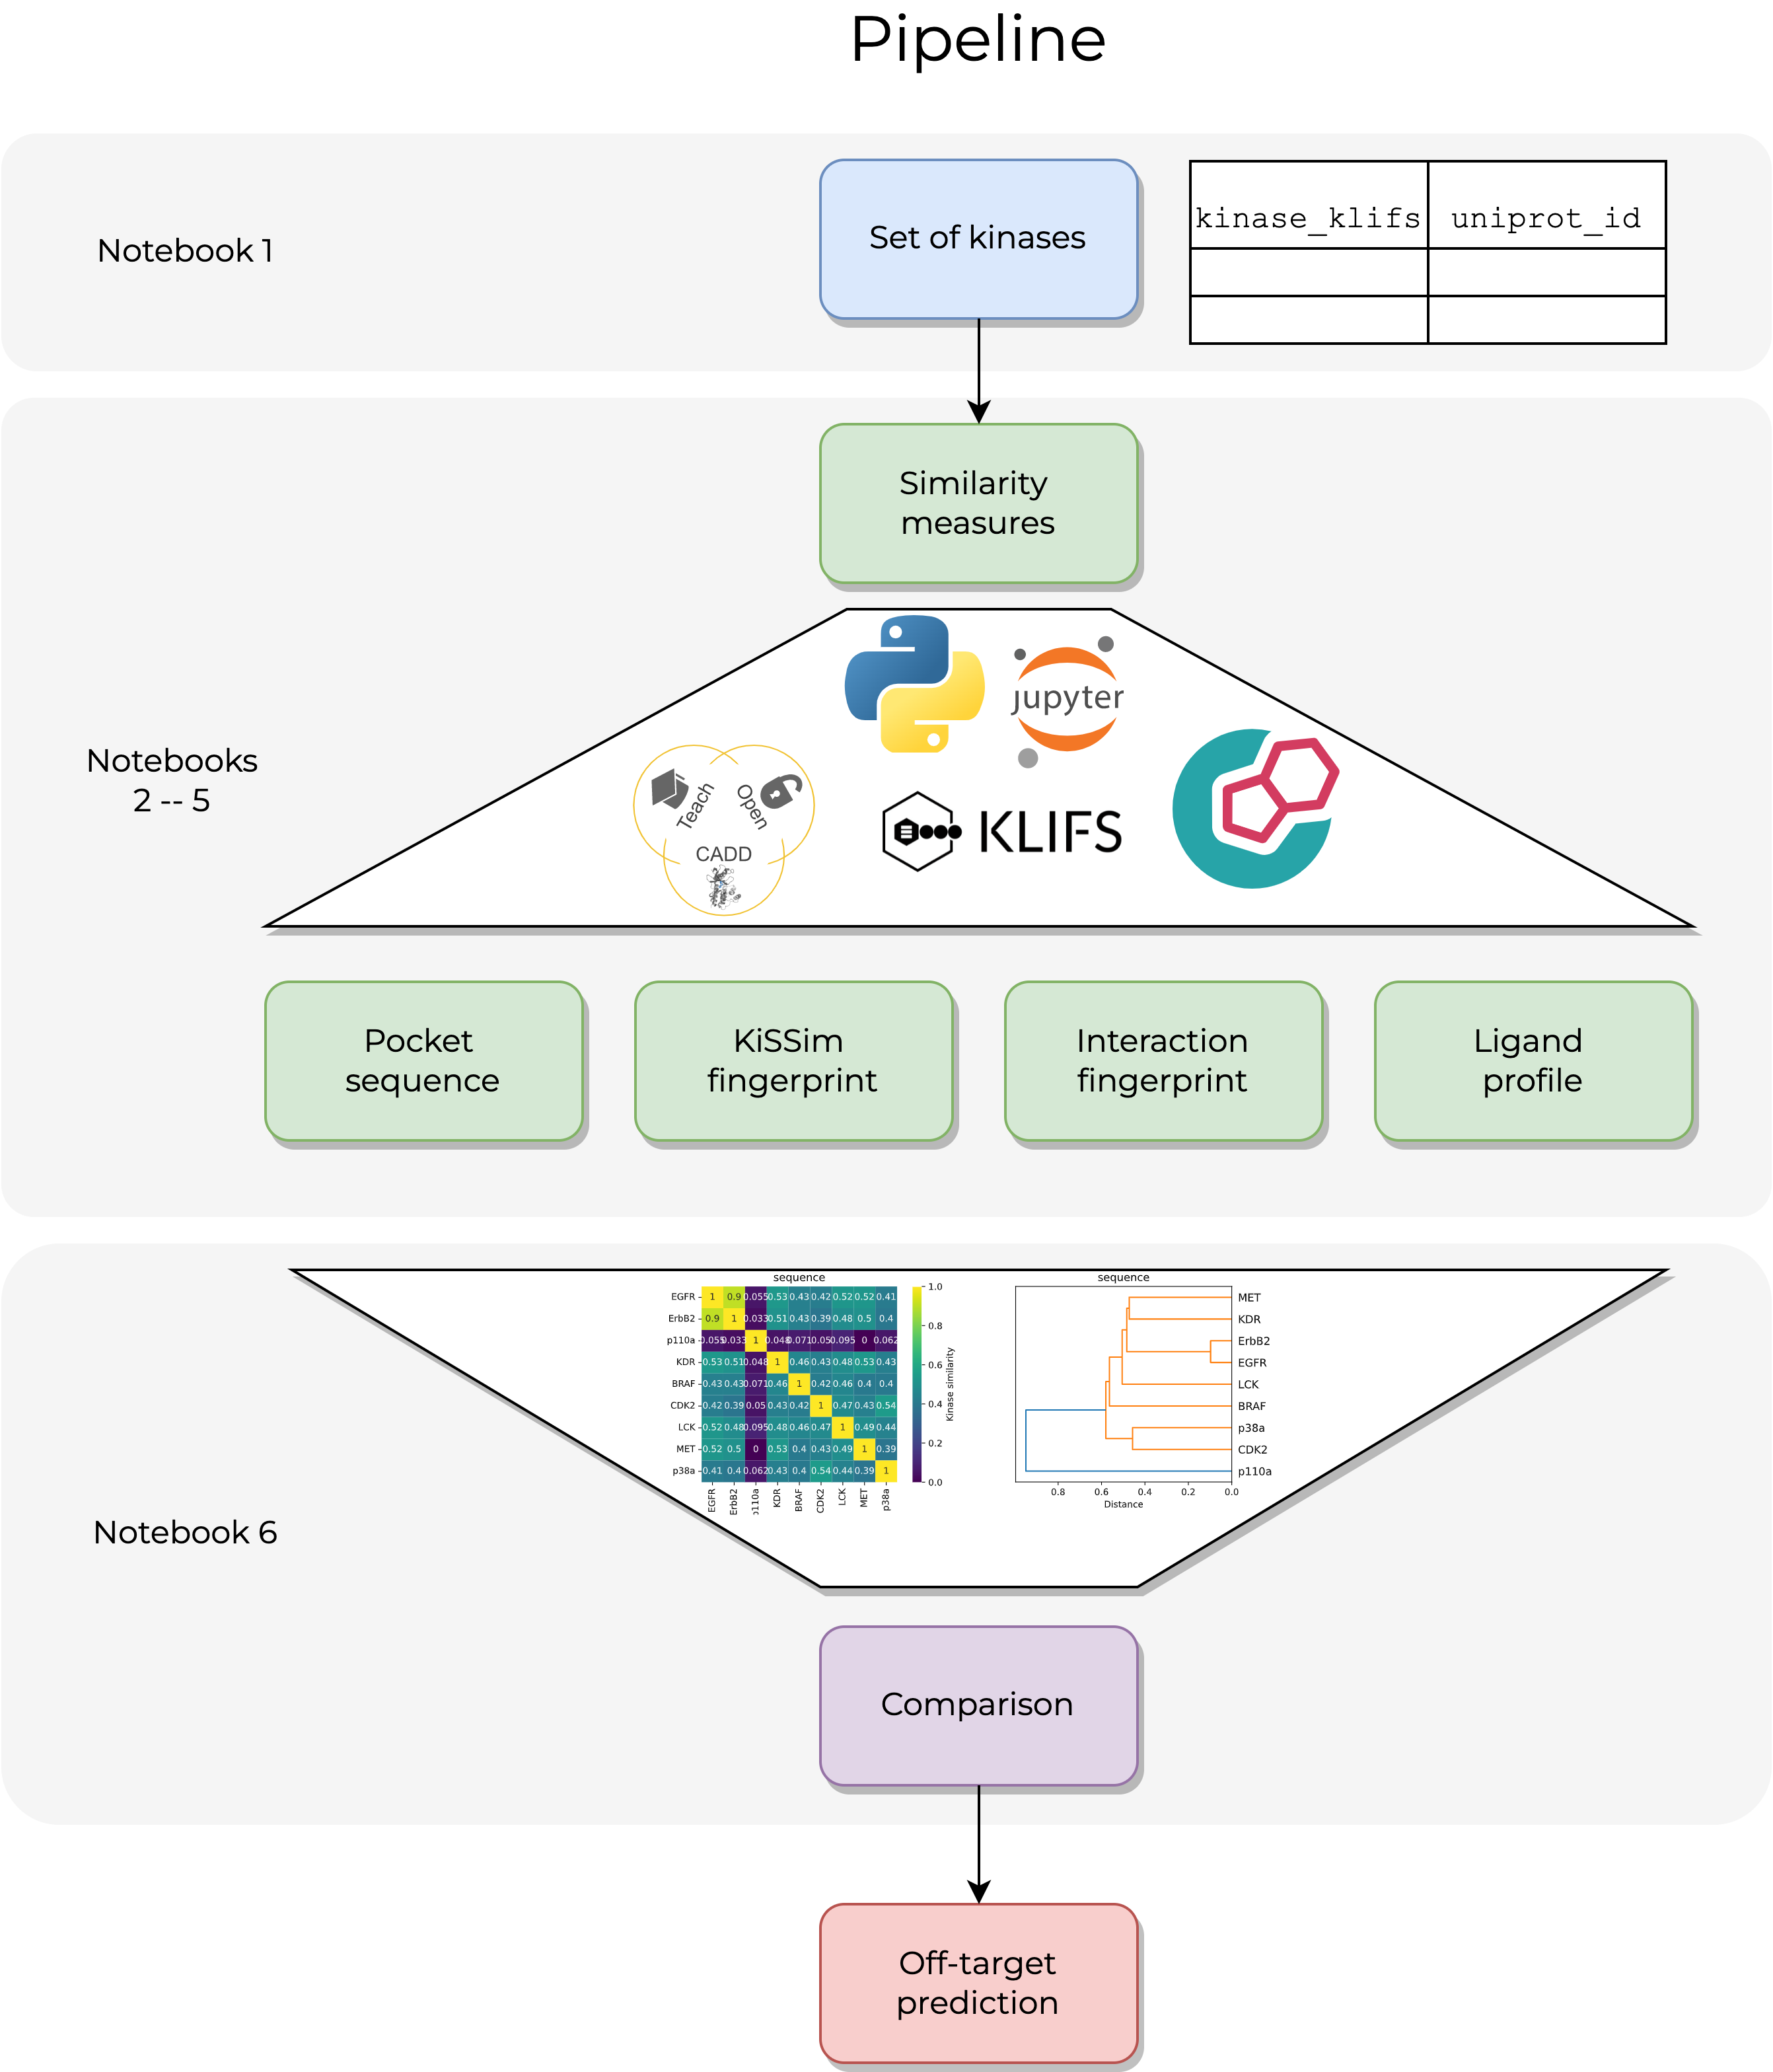
\includegraphics[width=\columnwidth]{Pipeline.png}
    \caption{The proposed pipeline consists of six Jupyter notebooks~\cite{Kluyver_2016_Jupyter}. Given a set of kinases in a CSV format, four similarity measures are implemented, and kinases are compared using heatmaps and dendrograms. The project is part of TeachOpenCADD~\cite{Sydow_2019_JCheminform, Sydow_2021_toc_chemrxiv} and uses open-source tools and databases such as KLIFS~\cite{Kanev_2020_NAR} and ChEMBL~\cite{Gaulton_2016_nar}.}
    \label{fig:pipeline}
\end{figure}

\subsection{Structure of the notebooks}
The structure of all notebooks is as follows: the first section covers the theory written in Markdown and summarizes the necessary concepts to understand the task. Relevant references are also mentioned. The second part of a notebook deals with the actual implementation of the task in a pedagogical manner, including motivation for practical steps and detailed comments on coding decisions. Finally, a discussion and a quiz section wrap up the notebook.
This structure is very well suited from a teaching perspective, since it contains both theory and hands on programming. The notebook can easily be used as a medium for a presentation, and it allows for self-study and usage in own research projects.

\subsection{About the code}
% Python and pythonic code
The programming part is done in Python exclusively and the code follows the latest software best practices. It is written pythonically and contains lots of code comments.
% reproducibility
Thanks to the continuous integration~(CI), all outputs and results are fully reproducible and the pipeline's maintenance is facilitated.

\subsection{Content of the pipeline}
As mentioned previously, the proposed pipeline contains six notebooks, described below:

The first notebook sets the stage with a kinase introduction and references/tools on where to find kinase-related information. It is also in this first notebook that a set of kinases of interest is defined. In this study, nine kinases are selected, the same nine as in the paper by \citet{Schmidt_2021_molecules}, where the authors discussed the challenges and advantages of tackling kinase similarities from multiple perspectives. Table~\ref{tab:kinase_selection} summarizes the information used for these kinases.
% Adaptable to other kinases
The pipeline can be executed out-of-the box with the defined set of kinases, but it can equally be run with a different user defined set of kinases. The only condition is that the uploaded CSV file with the kinases of interest contains two mandatory columns, namely \texttt{kinase\_klifs}, which is the KLIFS name of the kinase, and \texttt{uniprot\_id}, the Uniprot identifier~(ID)~\cite{uniprot_consortium_2020_nar} of the kinase (Figure~\ref{fig:pipeline}).

The four following notebooks describe one similarity method at a time as discussed in Section~\ref{sec:method}: the pocket sequence, the KiSSim fingerprint, the interaction fingerprint, and the ligand profile.

The final notebook collects the information from the previous ones and compares the different perspectives with easy-to-understand visualization such as heatmaps and dendrograms (see Section~\ref{sec:comparison}).

\subsection{Features of the pipeline}
The developed pipeline contains many useful features. Firstly, it is part of the TeachOpenCADD project~\cite{Sydow_2019_JCheminform, Sydow_2021_toc_chemrxiv} and extends it with this special kinase edition. Being part of TeachOpenCADD has the following advantages:
\begin{enumerate}
    \item TeachOpenCADD is open-source and freely available at \href{https://github.com/volkamerlab/teachopencadd}{https://github.com/volkamerlab/teachopencadd}, the project being licensed under the Attribution 4.0 International (CC BY 4.0).
    \item A dedicated conda package~\cite{conda_forge} facilitates installation.
    \item The teaching approach makes the notebooks easy to follow.
\end{enumerate}
Moreover, the pipeline is easily adaptable to new sets of kinases defined by an external user, as well as new similarity methods.

\begin{table*}
\centering
\begin{tabular}{lllll}
\hline
kinase & \textbf{kinase\_klifs} & \textbf{uniprot\_id} & group    & full kinase name                               \\
\hline
\hline
EGFR   & EGFR          & P00533      & TK       & Epidermal growth factor receptor                 \\
ErbB2  & ErbB2         & P04626      & TK       & Erythroblastic leukemia viral oncogene homolog 2 \\
PI3K   & p110a         & P42336      & Atypical & Phosphatidylinositol-3-kinase                    \\
VEGFR2 & KDR           & P35968      & TK       & Vascular endothelial growth factor receptor 2    \\
BRAF   & BRAF          & P15056      & TKL      & Rapidly accelerated fibrosarcoma isoform B       \\
CDK2   & CDK2          & P24941      & CMGC     & Cyclic-dependent kinase 2                        \\
LCK    & LCK           & P06239      & TK       & Lymphocyte-specific protein tyrosine kinase      \\
MET    & MET           & P08581      & TK       & Mesenchymal-epithelial transition factor         \\
p38a   & p38a          & Q16539      & CMGC     & p38 mitogen activated protein kinase alpha      \\
\hline
\end{tabular}
    \caption{Set of defined kinases. The table lists the kinases used in the pipeline, the same nine as in the study by \citet{Schmidt_2021_molecules}. It is noteworthy that the pipeline is applicable to an arbitrary set of kinases, the only condition being that the input CSV file should contain two columns, \texttt{kinase\_klifs} and \texttt{uniprot\_id}, displayed in bold.}
    \label{tab:kinase_selection}
\end{table*}

%A training article may on additional files and materials; clearly indicate where and how these are available, with links, and how they are being archived for the long-term and maintained so they stay current.
%You will likely want to reference your GitHub repository as a central point to access all of this information, and then the GitHub repository may link out to other content as needed.

\section{Conclusion}
In this study, a full pipeline for the assessment of kinase similarity is presented, using four methods of comparison. The pipeline is composed of six Jupyter notebooks:
\begin{enumerate}
    \item An introduction to kinases and their central role in drug discovery, as well as collecting the kinase set for the downstream notebooks.
    \item The similarity from a pocket sequence point of view.
    \item The similarity based on the KiSSim fingerprint, which encodes physico-chemical and spatial properties of the kinase pocket.
    \item The similarity based on KLIFS interaction fingerprints between the kinase pocket residues and a co-crystallized ligand.
    \item The similarity based on ligand profiling data collected from ChEMBL, measuring a compound's activity on a kinase.
    \item An analysis notebook which collects the proximity matrices calculated for the four methods, visualizes the similarities with heatmaps and the clusters with dendrograms, and finally discusses the results.
\end{enumerate}

We encourage users to develop their own similarity methods and to contribute to the existing pipeline.

This paper is a shout-out to
\begin{enumerate}
    \item researchers who want to gain insights into off-target prediction and kinase similarities, and integrate their new comparison methods to a working workflow,
    \item beginners in software development who need inspiration to set up a fully functional pipeline,
    \item teachers who want a starting point for lecture material,
    \item students with a background in bioinformatics, cheminformatics, and the life sciences in general,
    \item anyone who is curious.
\end{enumerate}



\section*{Author Contributions}
%%%%%%%%%%%%%%%%
% This section must describe the actual contributions of
% author. Since this is an electronic-only journal, there is
% no length limit when you describe the authors' contributions,
% so we recommend describing what they actually did rather than
% simply categorizing them in a small number of
% predefined roles as might be done in other journals.
%
% See the policies ``Policies on Authorship'' section of https://livecoms.github.io || https://livecomsjournal.github.io/authors/policies/ 
% for more information on deciding on authorship and author order.
%%%%%%%%%%%%%%%%

% following the CRediT taxonomy: https://www.cell.com/pb/assets/raw/shared/guidelines/CRediT-taxonomy.pdf
Conceptualization: TBK, DS, AV; Methodology: TBK, DS, AV; Software: TBK, DS, AV; Validation: TBK, DS, AV; Formal Analysis: TBK, DS, AV; Investigation: TBK, DS, AV; Writing -- Original Draft: TBK, DS, AV; Writing -- Review \& Editing: TBK, DS, AV; Visualization: TBK, DS, AV; Project Administration: TBK, DS, AV; Funding Acquisition, Supervision: AV.

% We suggest you preserve this comment:
For a more detailed description of author contributions,
see the GitHub issue tracking and changelog at \githubrepository.

%\section*{Other Contributions}
%%%%%%%%%%%%%%%
% You should include all people who have filed issues that were
% accepted into the paper, or that upon discussion altered what was in the paper.
% Multiple significant contributions might mean that the contributor
% should be moved to authorship at the discretion of the a
%
% See the policies ``Policies on Authorship'' section of https://livecoms.github.io for
% more information on deciding on authorship and author order.
%%%%%%%%%%%%%%%

%(Explain the contributions of any non-author contributors here)
% We suggest you preserve this comment:
%For a more detailed description of contributions from the community and others, see the GitHub issue tracking and changelog at \githubrepository.

\section*{Potentially Conflicting Interests}
%%%%%%%
%Declare any potentially competing interests, financial or otherwise
%%%%%%%

% Declare any potentially conflicting interests here, whether or not they pose an actual conflict in your view.
The authors declare no conflict of interests.

\section*{Abbreviations}
List of abbreviations used in the paper.
\begin{table}[H]
    \centering
    \begin{tabular}{l l}
        KLIFS & Kinase-Ligand Interaction Fingerprints and Structures\\
        EGFR & Epidermal Growth Factor Receptor\\
        KiSSim & Kinase Structure Similarity\\
        IFP & Interaction Fingerprint \\
        ID & Identifier\\
        CI & Continuous Integration
    \end{tabular}
\end{table}


\section*{Funding Information}
%%%%%%%
% Authors should acknowledge funding sources here. Reference specific grants.
%%%%%%%
TBK received funding from the Stiftung Charit\'e in the context of the Einstein BIH Visiting Fellow Project, DS from the Deutsche Forschungsgemeinschaft (grant VO 2353/1-1), and AV from the Bundesministerium f\"ur Bildung und Forschung (grant number 031A262C).

\section*{Author Information}
\makeorcid

\bibliography{bibliography}

%%%%%%%%%%%%%%%%%%%%%%%%%%%%%%%%%%%%%%%%%%%%%%%%%%%%%%%%%%%%
%%% APPENDICES
%%%%%%%%%%%%%%%%%%%%%%%%%%%%%%%%%%%%%%%%%%%%%%%%%%%%%%%%%%%%

%\appendix

\end{document}
